\documentclass[12pt]{article}

\usepackage{sbc-template}

\usepackage{graphicx,url}

\usepackage[brazil]{babel}
%\usepackage[latin1]{inputenc}
\usepackage[T1]{fontenc} % Selecao de codigos de fonte.
\usepackage[utf8]{inputenc} % Codificacao do documento (conversão automática dos acentos)
% UTF-8 encoding is recommended

\sloppy

\title{Aplicativo para Lista de Compras\\em um Comércio Varejista}

\author{Gilberto E. Tavares\inst{1}, Mário E. Augusto\inst{1}}

\address{Universidade do Estado de Santa Catarina (UDESC) -- São Bento do Sul, SC -- Brazil
  \email{mario.augusto@udesc.br, gilbertoetavares@gmail.com}
}

\usepackage[pdfauthor={Gilberto E. Tavares, Ma{'}rio E. Augusto},%
pdftitle={Aplicativo para Lista de Compras em um Com{\'e}rcio Varejista},%
pagebackref=true,%
pdftex]{hyperref}

\begin{document}

\maketitle

\begin{abstract}
  Abstract.
\end{abstract}

\begin{resumo}
  Resumo.
\end{resumo}


\section{Introdução}

Visando produtividade, eficiência e praticidade cada vez mais processos sãoautomatizados, nos mais diversos ramos e portes empresariais variando desde as menores até as grandes companhias. Essas automatizações proporcionam o autosserviço, que possibilita em toda hierarquia da equipe a descentralização de funções e informações.

Níveis de acesso e aprovação podem ser definidos, seguindo a política da empresa. Isso garante controle operacional, de modo autônomo e flexível, que simplifica aos envolvidos, a participação neste processos informatizados. Em acordo com o apoiador de pequenos negócio \cite{sebrae2015}, alguns benefícios dessa automatização são:

\begin{itemize}
\item Redução de custo no treinamento desses processos;
\item Possibilita execução com confiança e consistência;
\item Torna ágil as atividades, com aperfeiçoamento e mudança gradual;
\item Mantêm diretrizes, por estar definido na implementação.
\end{itemize}

\section{Justificativa}

Na investigação desses processos pré-estabelecidos na empresa Alecrim Dourado Variedades, foi encontrado de modo oportuno a atividade visual e de registro, de todas mercadorias que devem obtidas no mercado atacadista. O processo manual, centralizado e sem controle apropriado, é realizado através da clássica planilha eletrônica. Esta realidade propicia através do desenvolvimento de aplicação própria uma evolução tangível.

Durante a análise alguns pontos foram verificados como motivacionais à criação do sistema informacional proposto, tendo soluções relativas:

\begin{itemize}
\item Acesso centralizado da informação;
\item Informação imediata;
\item Registro de item com funcionário e data;
\item Redução de retrabalho;
\item Menor índice de duplicidade de itens;
\item Possibilidade de não utilização de impressão em papel.
\end{itemize}

\section{Objetivos}

Desenvolvimento de aplicação para gerir itens em lista de compras, também o acompanhamento durante a compra dos mesmos. Devendo este aplicativo ser acessível em dispositivos móveis, com devido tratamento em casos de indisponibilidade de conectividade.

\section{Modelo Inicial}

A empresa do estudo é classificada como varejista, comercializa produtos variados: papelaria, utilidades, ferramentas, vestuário, brinquedos, info-eletrônicos, decoração, doces e outros.

O costumeiro é que cada funcionária tenha sempre consigo uma caderneta (no bolso do colete fornecido pela loja) e anote itens que são de sua seção assim que seja percebida a necessidade. Entende-se como necessidade: (\textit{i}) itens que ainda não sejam comercializados anteriormente, mas que um ou mais clientes demonstrem interesse e sejam pertinentes dentro da proposta de loja; (\textit{ii}) itens já comercializadas mas que tenham acabado ou estejam por acabar, bem como possa seu estoque não durar até a próxima compra.

Não é regra ou obrigatório anotar somente itens da seção a qual a funcionária é responsável, muito pelo contrário, prefere-se que seja assim pois antes ``pecar'' pelo excesso que pela falta, será pior um item não ter sido anotado do que estar repetido em listas diferentes. Pois na próxima etapa deve o digitador filtrar para que não permanecem itens duplicados, porém essa ação tem complicação por itens com nomes dúbios (descritos com termos diferentes) ou mesmo quando compostos por várias palavras podem estar em várias ordem ou abreviações.

Utiliza-se um arquivo `pasta de planilha eletrônica' do Microsoft Excel. A planilha utilizada é bem simples, como pode ser visto na Figura  \ref{fig:planilha}, não há fórmulas ou macros, são apenas três colunas nas quais os itens são preenchidos conforme sua classificação. Essa essa classificação diz respeito ao local em que será comprada a mercadoria, pois alguns tipos são melhor encontrados em lojas especializadas. Segue a categorização utilizada:

\begin{itemize}
\item \textbf{Atacado}: são itens comprados os em três grandes lojas atacadistas. É considerada a principal por ter o de maior volume no registro, após formatada a lista para impressão apresenta-se em três colunas. Tem-se como título dessa coluna \textbf{Item};
\item \textbf{Info-eletrônicos}: itens como cabos, fones, carregadores, pilhas, rádios, controle remoto, etc. São encontrados em lojas em ruas populares no comércio deste segmento. Seu título consta como \textbf{SP}, na impressão varia entre uma a duas colunas;
\item \textbf{Bijuterias e acessórios}: itens como maquiagens, bijuterias, acessórios, bonés, bolsas, etc. São também encontrados no comércio popular e em um dos atacados visitados. Sua coluna indica \textbf{Bijuterias/Acessórios}, na impressão uma coluna é suficiente.
\end{itemize}

\begin{figure}[ht]
\caption{Planilha utilizada}\label{fig:planilha}
\centering
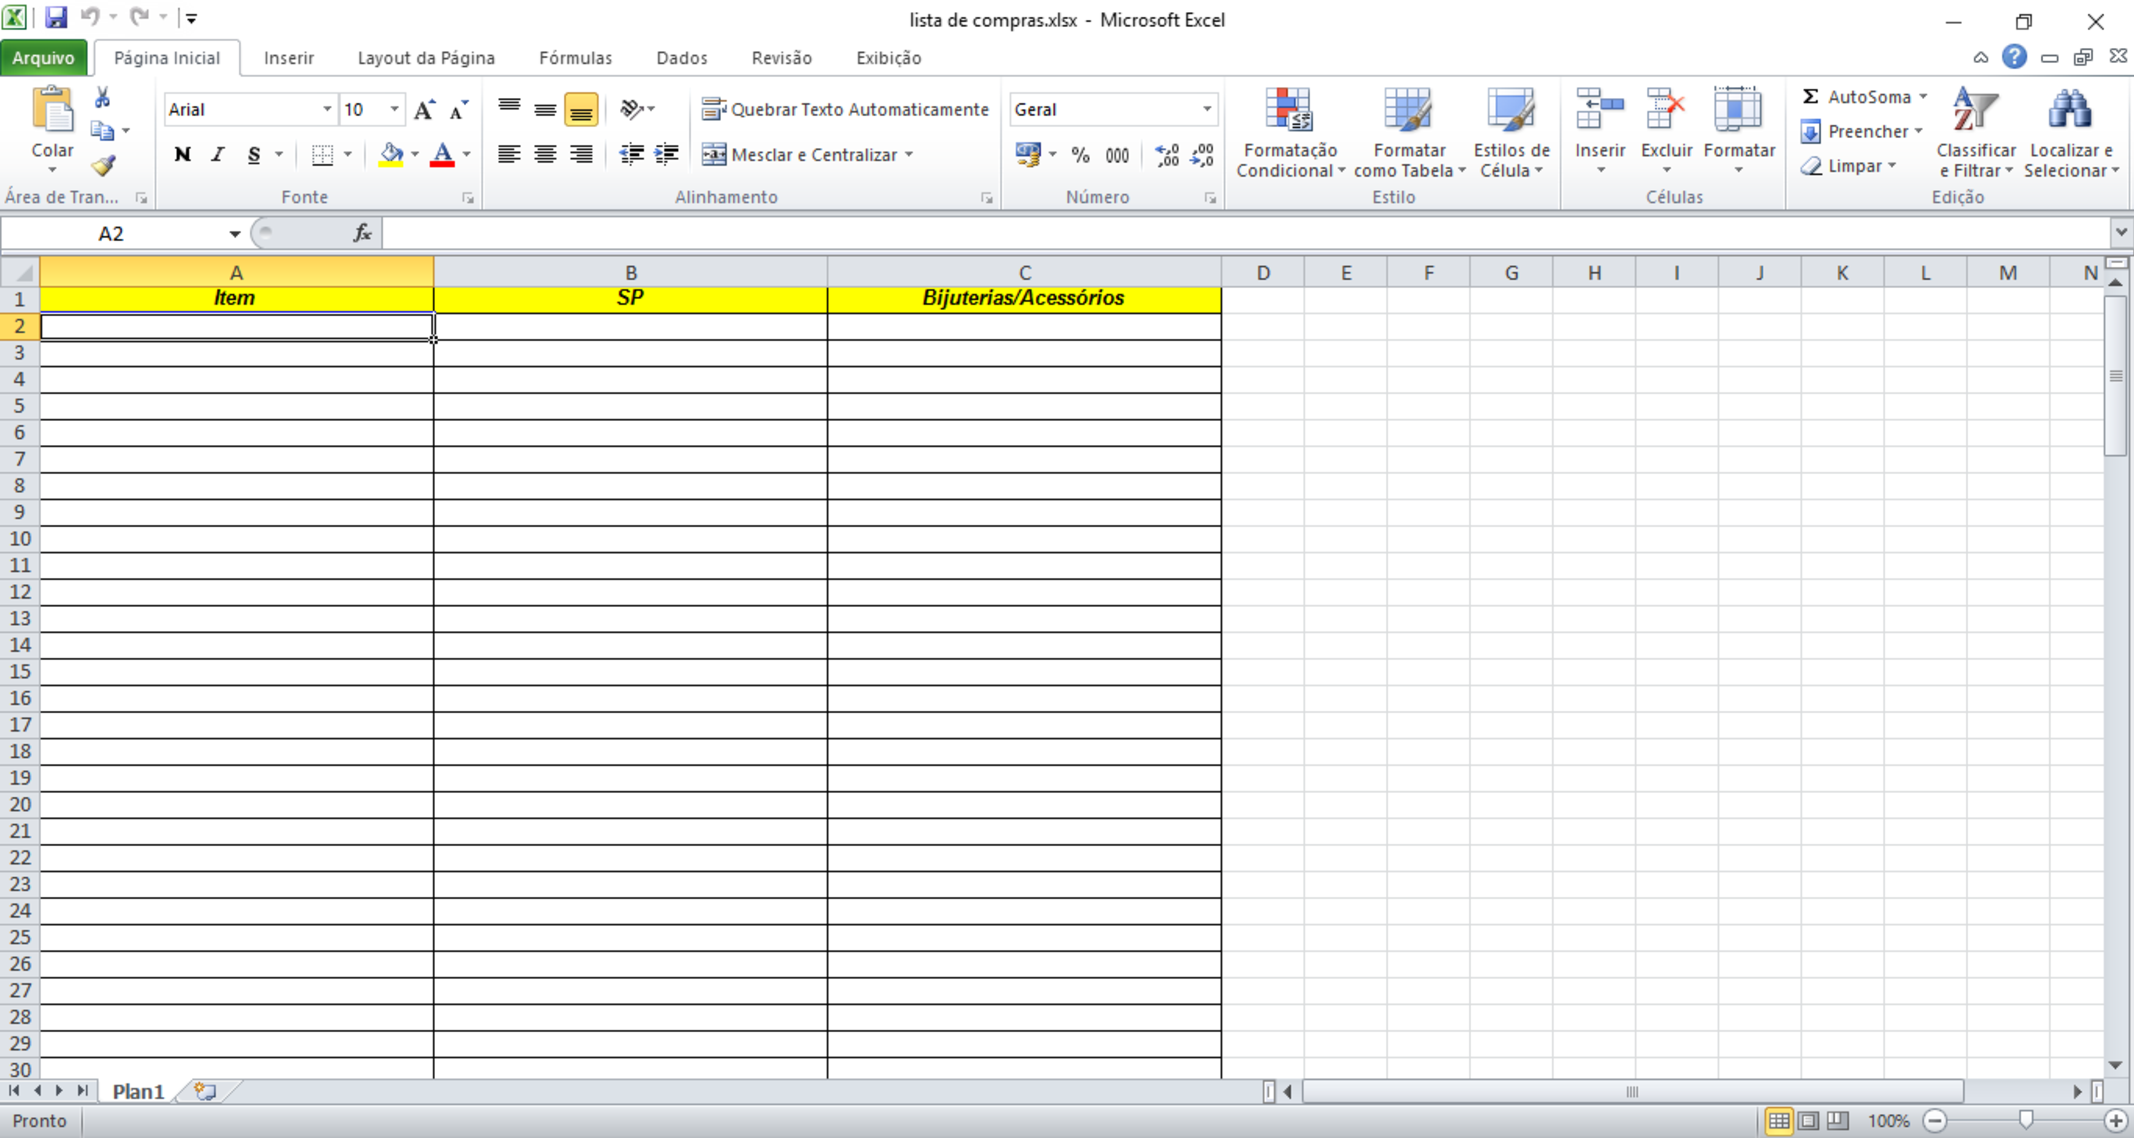
\includegraphics[width=\textwidth,keepaspectratio]{figures/lista-excel.pdf}
\caption*{\footnotesize Fonte: Produção do autor, 2016.}
\end{figure}

Quando no processo de compras esta lista é levada impressa congorme Figura \ref{fig:impressao}.

\begin{figure}[ht]
\caption{Modelo de Impressão da Planilha}\label{fig:impressao}
\centering
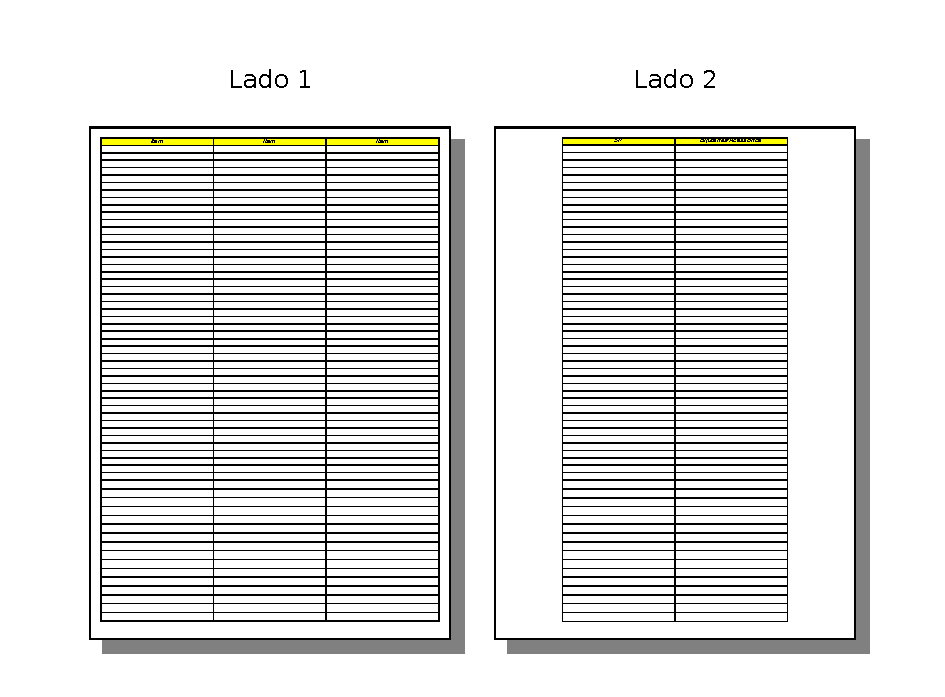
\includegraphics[width=\textwidth,keepaspectratio]{figures/modelo-impressao.pdf}
\caption*{\footnotesize Fonte: Produção do autor, 2016.}
\end{figure}

\bibliographystyle{sbc}
\bibliography{references}

\end{document}
